\documentclass[bigger]{beamer}
\usepackage[utf8]{inputenc}
\usepackage{hyperref}
\usepackage{ragged2e} 
\usepackage{listingsutf8}
\usepackage[normalem]{ulem}
\usepackage{graphicx}
\usepackage{transparent}
\usepackage[absolute,overlay]{textpos}
\usepackage{todonotes}
\usepackage[spanish,es-tabla]{babel}
\usepackage[normalem]{ulem}

\definecolor{codegreen}{rgb}{0,0.6,0}
\definecolor{codegray}{rgb}{0.5,0.5,0.5}
\definecolor{codepurple}{rgb}{0.58,0,0.82}
\definecolor{backcolour}{rgb}{0.95,0.95,0.92}



\lstdefinestyle{mystyle}{
	backgroundcolor=\color{backcolour},
	commentstyle=\color{codegreen},
	keywordstyle=\color{magenta},
	numberstyle=\tiny\color{codegray},
	stringstyle=\color{codepurple},
	basicstyle=\tiny,
	breakatwhitespace=false,
	breaklines=true,
	captionpos=b,
	keepspaces=true,
	numbers=left,
	numbersep=5pt,
	showspaces=false,
	showstringspaces=false,
	showtabs=false,
	tabsize=2
}

\lstset{style=mystyle}

%tema de las trapas
%\usetheme{Berlin}
\usetheme{metropolis}
%\usecolortheme{beaver}


\newcommand{\tab}[1]{\hspace{.2\textwidth}\rlap{#1}}

\title{Wakamola}
\subtitle{Primer piloto en Tavernes} 
\author[IBIME]{Vicent Blanes Selva}
\date{01/02/2019}

\setbeamertemplate{footline}[frame number]

%comienzo documento
\begin{document}
	%empezamos con el primer frame
	%{\usebackgroundtemplate%
		%
		%{\transparent{0.2}\includegraphics[width=\paperwidth,height=\paperheight]{img/fondo.jpg}}%
	\begin{frame}
		\titlepage
	\end{frame}
	%}

\begin{frame}{Introducción}
\begin{columns}[T]
	% columna izquierda
	\begin{column}[T]{6cm}
		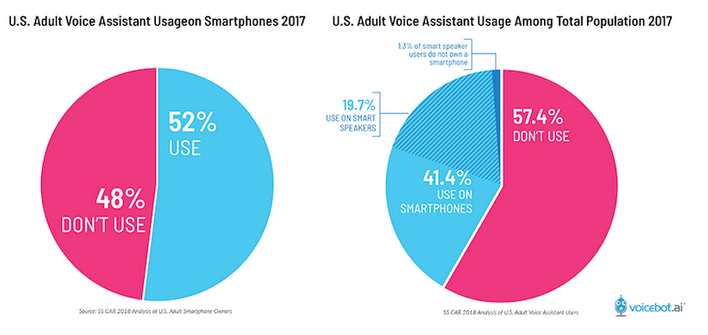
\includegraphics[scale=0.35]{img/usage1}
		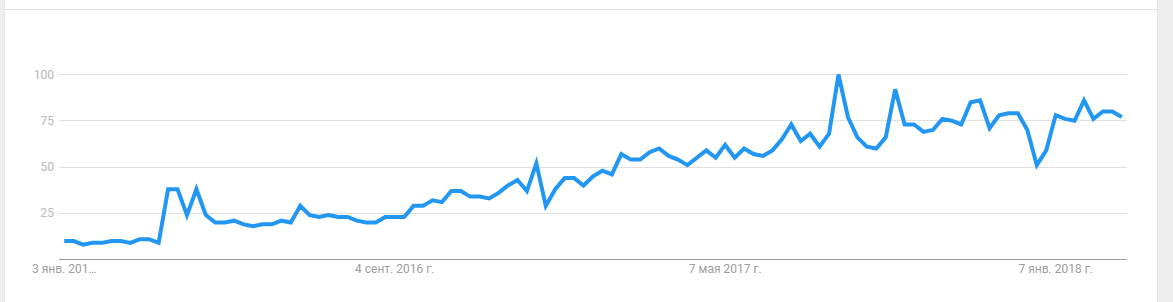
\includegraphics[scale=0.30]{img/usage4}
		
	\end{column}
	\begin{column}[T]{5.5cm}
		\raggedright
		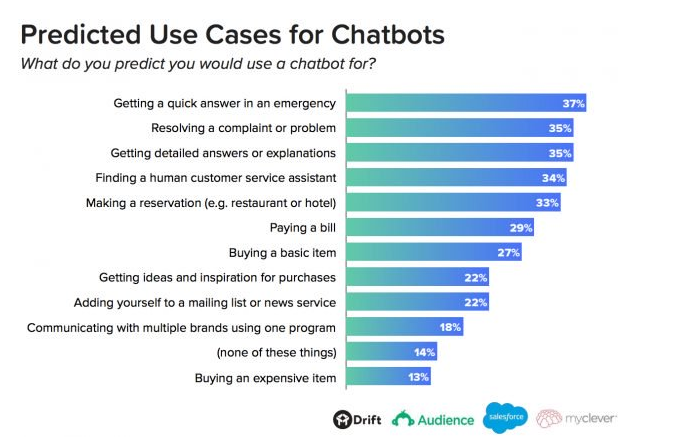
\includegraphics[scale=0.3]{img/usage3}
	\end{column}
\end{columns}	
\end{frame}

\begin{frame}{¿Qué es Wakamola?}
	\centering
	
\includegraphics[scale=0.95]{img/wakamola_logo}\\
	Piloto en Tavernes:\textbf{ @WakamolatavernesBot}
\end{frame}

\begin{frame}{Componentes de Wakamola}
	% columnas, teclado a la derecha y explicación a la izquierda
	\begin{columns}[T]
		% columna izquierda
		\begin{column}[T]{6cm}
			\centering
			\vspace{0.1cm}
			\begin{itemize}
				\item Encuesta personal*
				\item Encuesta sobre alimentación (CFCA validado)*
				\item Encuesta actividad física: IPAQ corto
				\item Mecanismo para compartir
				\item Wakaestado
			\end{itemize}
		\tiny
		\textit{*Preguntas añadidas/modificadas desde La Fe o la UV}
		\end{column}
		% columna derecha
		\begin{column}[T]{6cm}
			\centering
			% imagen de python y mariadb
			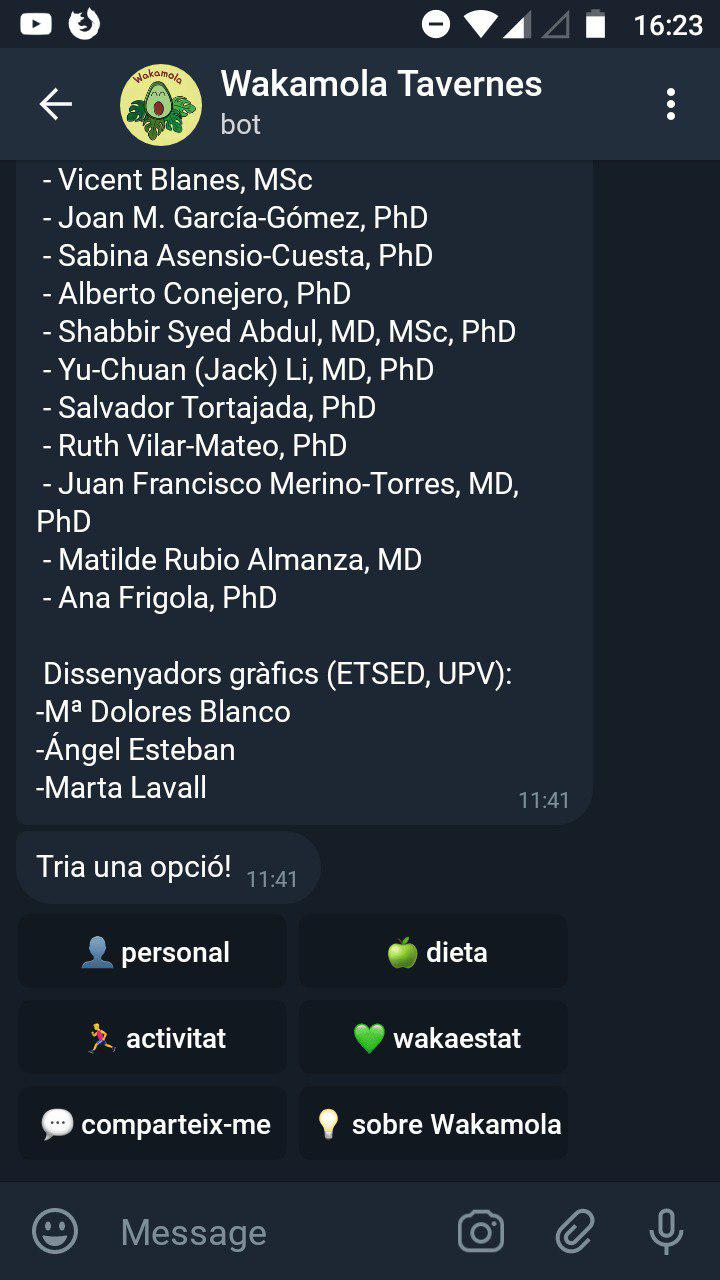
\includegraphics[scale=0.15]{img/teclado}
		\end{column}
	\end{columns}
 \end{frame}

\begin{frame}{Componentes de Wakamola: Wakaestado}
	\begin{columns}[T]
		\begin{column}[T]{6cm}
		\centering
		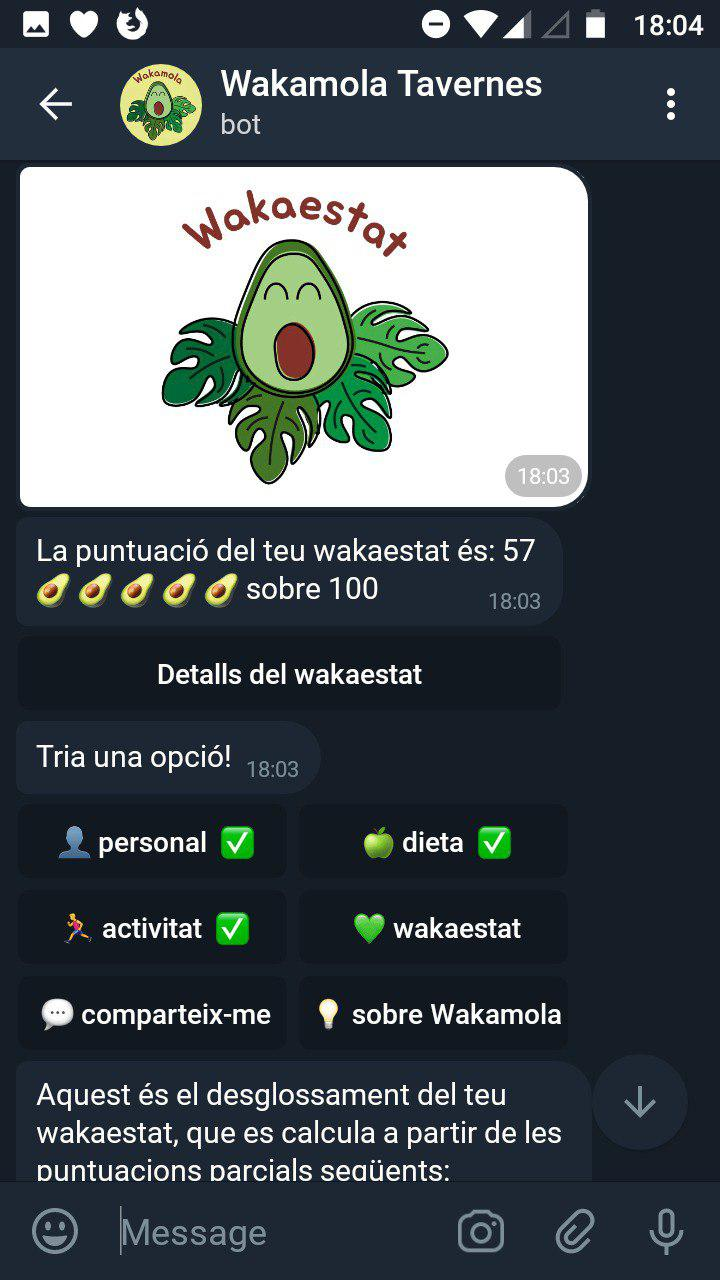
\includegraphics[scale=0.16]{img/wakaestado}
		\end{column}
		% columna derecha
		\begin{column}[T]{6cm}
		\centering
		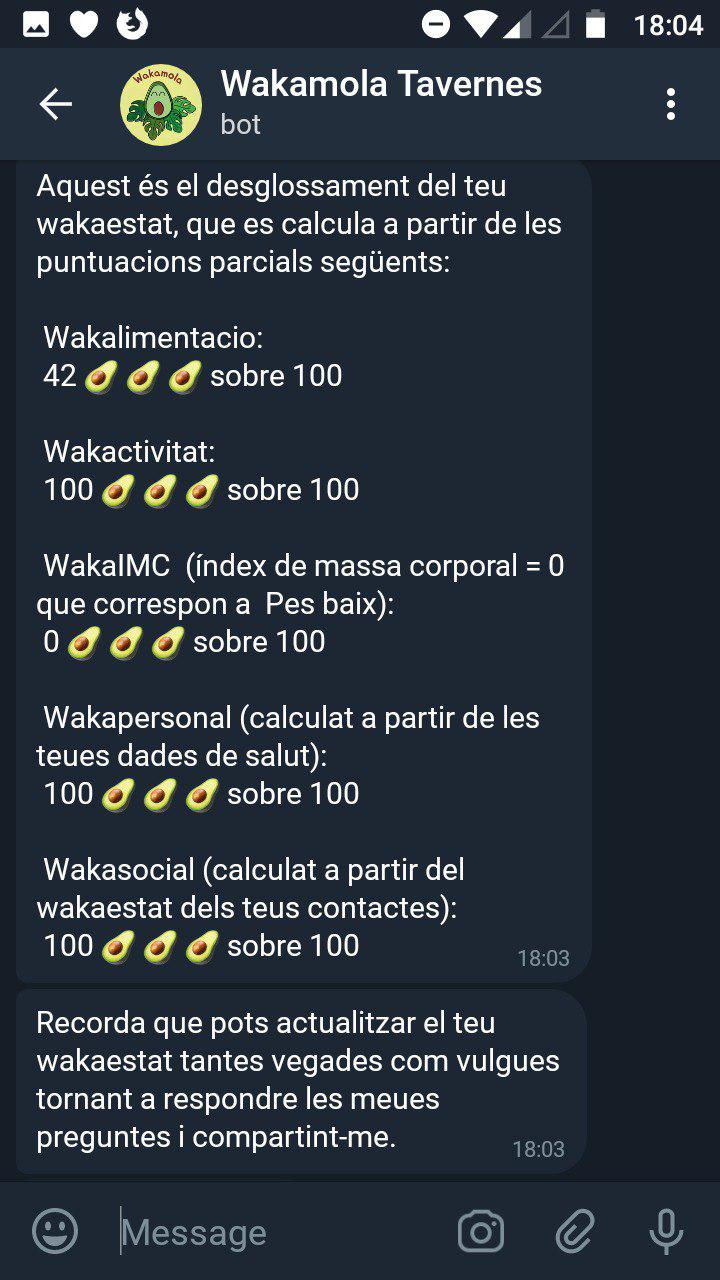
\includegraphics[scale=0.16]{img/wakaestadodetail}
		\end{column}
\end{columns}
\end{frame}

\begin{frame}{Componentes de Wakamola: Red Social}
\begin{columns}[T]
	\begin{column}[T]{6cm}
		\centering
		\vspace{0.2cm}
		\begin{itemize}
			\item Inspirado en un estudio de obesidad de Framingham
			\item Objetivo: \textbf{Estudiar influencia de la red social y el entorno}
			\item Debido a la seguridad de Telegram, la manera más efectiva de compartir es utilizar \textit{deep linking} 
		\end{itemize}
	\end{column}
	% columna derecha
	\begin{column}[T]{6cm}
		\centering
		
\includegraphics[scale=0.16]{img/social}
	\end{column}
\end{columns}
\end{frame}

\begin{frame}{¿Como funciona? (Perspectiva BOT)}
	\centering
	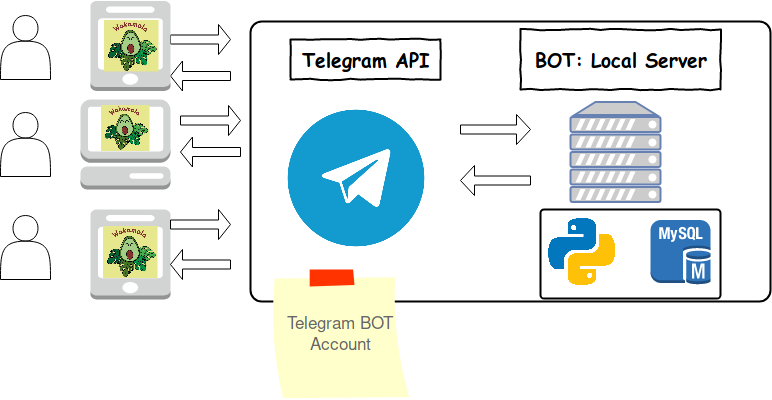
\includegraphics[scale=0.4]{img/diagramawakamola}
\end{frame}

\begin{frame} {¿Como funciona? (Tecnologías)}
	\begin{columns}[T]
		% columna izquierda
		\begin{column}[T]{6cm}
			\centering
			\vspace{1.9cm}
			\begin{itemize}
				\item Python
				\vspace{0.1cm}
				\item MariaDB
				\vspace{0.1cm}
				\item Networkx (librería)
				\vspace{0.1cm}
				\item Cytoscape (Visualización)
			\end{itemize}
		\end{column}
		% columna derecha
		\begin{column}[T]{6cm}
			\centering
			% imagen de python y mariadb
			
\includegraphics[scale=0.2]{img/python}
			
\includegraphics[scale=0.2]{img/mariadb}
		\end{column}
	\end{columns}
\end{frame}

\begin{frame}{Seguridad}
	\begin{itemize}
		\item Los bots no pueden acceder al número de teléfono de ningún usuario
		\item Se utiliza un sistema de IDs que no tiene correlación con los datos del usuarios
		\item El bot debe ser activado previamente por el usuario (para evitar spam)
		\item Telegram utiliza cifrado entre el servidor y los dispositivos.
		\item La información en el servidor continua encriptada con varias claves repartidas alrededor del mundo. (\textit{declaración de Telegram})
		\item Wakamola utiliza una versión \textbf{hasheada} (con MD5) del ID de Telegram. El ID es convertido en una cadena alfanumérica de 128 bits. No es reversible.
	\end{itemize}
\end{frame}

\begin{frame}{Impacto: Usuarios}
	Datos actualizados en: \textbf{01/02/2019}
	\centering
	\begin{tabular}{c | c}
		Categoría & Nº Personas\\
		\hline\hline
		Usuarios totales (bot iniciado) & 287\\
		Han respondido personal & 192\\
		Han respondido alimentación & 164\\
		Han respondido actividad física & 162\\
		Todas las preguntas & 155\\
		\hline\hline
		
	\end{tabular}
\end{frame}

\begin{frame}{Impacto: administraciones y medios}
	\centering
	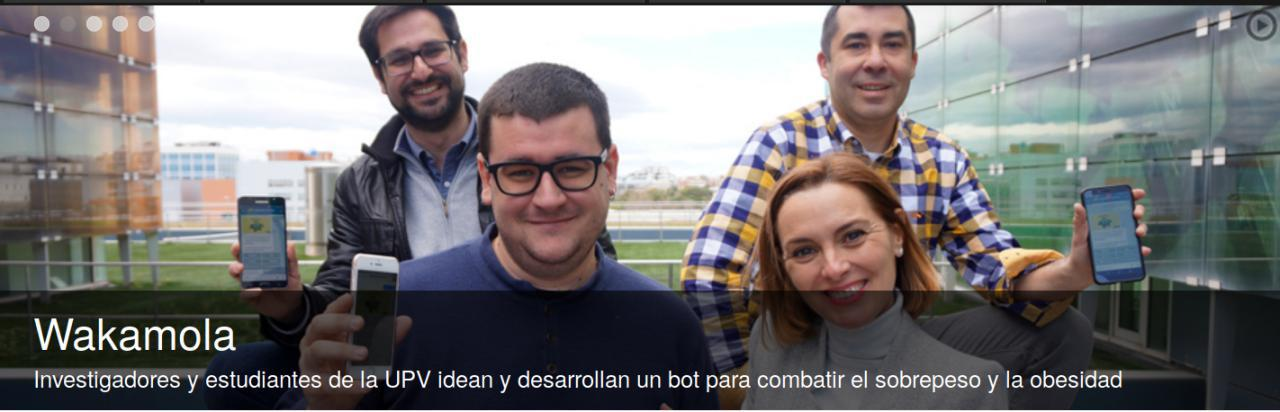
\includegraphics[scale=0.3]{img/prensa}
	\begin{itemize}
		\item Nota de prensa/entrevistas en varios medios: À punt, Cadena SER, El Periodic, 20 Minutos, Europapress...
		\item Interés mostrado por parte de diversos agentes en salud
	\end{itemize}
\end{frame}

\begin{frame}{Posibles mejoras}
	\begin{enumerate}
		\item Incremento de gamificación (contenido)
		\item Implementación Docker (técnica)
		\item Escalabilidad (técnica)
		\item Aplicación de NLP (técnica/contenido)
	\end{enumerate}
\end{frame}

\begin{frame}{Conclusiones}
	
\end{frame}

\begin{frame}{Enlaces de Interés}
	\begin{itemize}
	\item \href{https://voicebot.ai/2018/04/03/over-half-of-smartphone-owners-use-voice-assistants-siri-leads-the-pack/}{Gráfico de tarta introducción}
	\item \href{https://www.convinceandconvert.com/digital-marketing/6-critical-chatbot-statistics-for-2018/}{Gráfico de barras introducción}
	\item \href{https://chatbotsmagazine.com/chatbot-report-2018-global-trends-and-analysis-4d8bbe4d924b}{Gráfico tendencias de Google introducción}
	\item \href{https://www.nejm.org/doi/full/10.1056/nejme078114}{Estudio Framingham}
	\item \href{http://www.nutricionhospitalaria.com/pdf/4035.pdf}{CFCA Original}
	\item\href{https://youthrex.com/wp-content/uploads/2017/06/IPAQ-TM.pdf}{Cuestionario actividad física}
	\item\href{https://github.com/vblanes/alphahealth}{Repositorio público del proyecto}
	\end{itemize}
\end{frame}

\end{document}